%%%%%%%%%%%%%%%%%%%%%%%%%%%%%%%%%%%%%%%%%%%%%%
%                                            %
%   W Z O R Z E C   S P R A W O Z D A N I A  %
%                                            %
%%%%%%%%%%%%%%%%%%%%%%%%%%%%%%%%%%%%%%%%%%%%%%

% !TeX spellcheck = en_EN
\documentclass[12pt,a4paper]{article}

\usepackage{amsmath,amssymb}
\usepackage[utf8]{inputenc}                                      
\usepackage[OT4]{fontenc}      
%\usepackage[T1]{fontenc}    
%\usepackage{polski}                                                 
\usepackage{indentfirst} 
\usepackage[dvips]{graphicx}
\usepackage{tabularx}
\usepackage{color}
\usepackage{float}
\usepackage{hyperref} 
\usepackage{fancyhdr}
\usepackage{listings}
\usepackage{booktabs}
\usepackage{ifpdf}
\usepackage{mathtext} % polskie znaki w trybie matematycznym
%\makeindex  % utworzenie skorowidza (w dokumencie pdf)
\usepackage{lmodern}
%\usepackage[osf]{libertine}
\usepackage{filecontents}
\usepackage{bchart}
\usepackage{caption,subcaption}

\usepackage{tikz}
\usetikzlibrary{arrows}


\newcounter{nextYear}
\setcounter{nextYear}{\the\year}
\stepcounter{nextYear}

% rozszerzenie nieco strony
%\setlength{\topmargin}{-1cm} \setlength{\textheight}{24.5cm}
%\setlength{\textwidth}{17cm} \addtolength{\hoffset}{-1.5cm}
%\setlength{\parindent}{0.5cm} \setlength{\footskip}{2cm}
%\linespread{1.2} % odstep pomiedzy wierszami

\ifpdf
\DeclareGraphicsRule{*}{mps}{*}{}
\fi


\newcommand{\tl}[1]{\textbf{#1}} 
\pagestyle{fancy}
\renewcommand{\sectionmark}[1]{\markright{\thesection\ #1}}
\fancyhf{} % usuwanie bieżących ustawień
\fancyhead[LE,RO]{\small\bfseries\thepage}
\fancyhead[LO]{\small\bfseries\rightmark}
\fancyhead[RE]{\small\bfseries\leftmark}
\renewcommand{\headrulewidth}{0.5pt}
\renewcommand{\footrulewidth}{0pt}
\addtolength{\headheight}{0.5pt} % pionowy odstęp na kreskę
\fancypagestyle{plain}{%
\fancyhead{} % usuń p. górne na stronach pozbawionych numeracji
\renewcommand{\headrulewidth}{0pt} % pozioma kreska
}

% ustawienia listingu programow
%\lstset{	language=C++, 
%        	numbers=left, 
%        	numberstyle=\tiny, 
%        	stepnumber=1, 
%        	numbersep=5pt,
%		  	stringstyle=\ttfamily,
%			showstringspaces=false,
% 			tabsize=4
%		}

\lstset{%
language=C++,%
commentstyle=\textit,%
identifierstyle=\textsf,%
keywordstyle=\sffamily\bfseries, %
%captionpos=b,%
tabsize=3,%
frame=lines,%
numbers=left,%
numberstyle=\tiny,%
numbersep=5pt,%
breaklines=true,%
morekeywords={Student,Reg,Mark,string},%
escapeinside={(*@}{@*)},%
%basicstyle=\footnotesize,%
%keywords={double,int,for,if,return,vector,matrix,void,public,class,string,%
%float,sizeof,char,FILE,while,do,const}
}
%%%%%%%%%%%%%%%%%%%%%%%%%%%%%%%%%%%%%%%%%%%%%%%%%%%%%%%%%%%%%%%%%%%%%%%

% mala zmiana sposobu wyswietlania notek bocznych
\let\oldmarginpar\marginpar
\renewcommand\marginpar[1]{%
  {\linespread{0.85}\normalfont\scriptsize%
%   \oldmarginpar[\vspace{-1.5ex}\raggedleft\scriptsize\color{black}\textsf{#1}]%    left pages
%                {\vspace{-1.5ex}\raggedright\scriptsize\color{black}\textsf{#1}}% right pades
\oldmarginpar[\hspace{1cm}\begin{minipage}{3cm}\raggedleft\scriptsize\color{black}\textsf{#1}\end{minipage}]%    left pages
{\hspace{0cm}\begin{minipage}{3cm}\raggedright\scriptsize\color{black}\textsf{#1}\end{minipage}}% right pages
}%
}
% % % % % % % % % % % % % % % % % % % % % % % % % % % % % % % %

\begin{document}
\frenchspacing
\thispagestyle{empty}
\begin{center}
{\Large\sf Silesian University of Technology   % Alma Mater

Institute of Informatics

}

\vfill


\includegraphics[width=0.30\textwidth]{images/polsl}

\vfill\vfill

{\Huge\sffamily\bfseries Biologically Inspired Artificial Iintelligence} \\ % tu podać nazwę przedmiotu

\vfill\vfill

{\LARGE\sf Program for lossy compresing images with usage of self-organizng map(Kohonen SOM)}  % a tu temat laborki :-)


\vfill \vfill\vfill\vfill

%%%%%%%%%%%%%%%%%%%%%%%%%%%%


\begin{tabular}{ll}
\toprule
	author                 						   & Marek Żabiałowicz         	\\	
	e-mail                 						   & marekzabialowicz@gmail.com        	\\	
	teacher                                             & D.E. Grzegorz Baron			\\
	academic year                                         & 2018/2019					 \\
	study type                                         & SSI					 \\
	major                                               & Computer Science             \\
	semester                                                & 6                           \\
	group                                                  & GkiO4                        \\
	section                                                 & 9                           \\  
\bottomrule &  \\
\end{tabular}

\end{center}
%%%%%%%%%%%%%
%%%%%%%%%%%%%%%%%%%%%%%%%%%%%%%%%%%%%%%%%%%%%%%%%%%%%%%%%%%%%%%%%%%%%%%%%
\cleardoublepage
%%%%%%%%%%%%%%%%%%%%%%%%%%%%%%%%%%%%%%%%%%%%%%%%%%%%%%%%%%%%%%%%%%%%%%%%%

%%%%%%%%%%%%%%%%%%%%%%%%%%%%%%%%%%%%%%%%%%%%%%%%%%%%%%%%%%%%%%%%%%%%%%%%%
\section{Introduction}
The aim of my project was to write a program for lossy compresing images with usage of self-organizng map(Kohonen SOM) with implementaion one or a couple alghoritims: Winner Takes All, Winner takes Most, Soft Competition Scheme, Stochastic Relaxation, Neuron Gas.

\section{External specification}
The program use graphical window. With usage of buttons and sliders user can upload an image, set up lattice width and height, compress the image and save the image.

\begin{figure}[H]
\centering
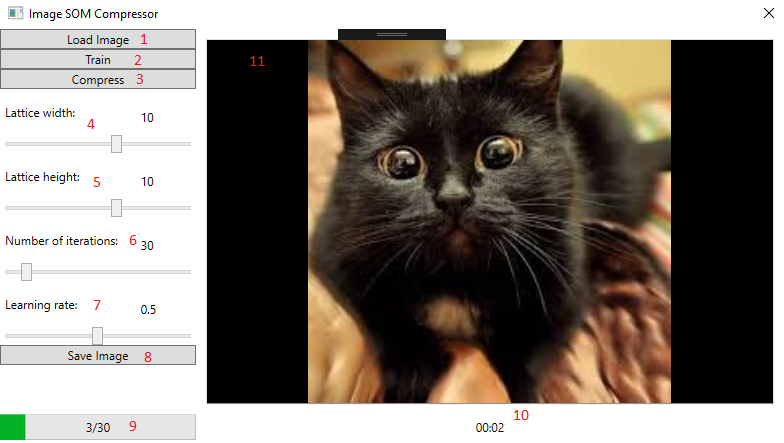
\includegraphics[width=\textwidth]{images/userInterface}
\caption{User interface}
\end{figure}

1 - load an image\\
2 - train self-organizng map\\
3 - compress an image\\
4 - setting latice width\\
5 - setting lattice height\\
6 - setting number of iterations\\
7 - setting a learning rate\\
8 - save an image\\
9 - progeress bar with number of current iteration\\
10 - elapsed time to learn\\
11 - preview of an image(before and after compressing)\\

\section{Internal specification}
Dzięki dobrej organizacji pracy sekcji, nie mieliśmy problemu z przesyłaniem między sobą danych. Na samym początku ustaliliśmy kolejność i typ danych, więc szybko mogliśmy zając się tworzeniem programu i wizualizacji.
    
\begin{figure}[htb]
    \centering % <-- added
\begin{subfigure}{0.25\textwidth}
  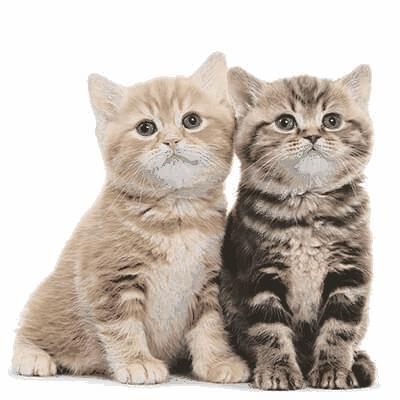
\includegraphics[width=\linewidth]{images/big/original}
  \caption{oryginal}
  \label{fig:1}
\end{subfigure}\hfil % <-- added
\begin{subfigure}{0.25\textwidth}
  
\includegraphics[width=\linewidth]{images/big/3-3-5-05}
  \caption{3x3 5 0.5}
  \label{fig:2}
\end{subfigure}\hfil % <-- added
\begin{subfigure}{0.25\textwidth}
  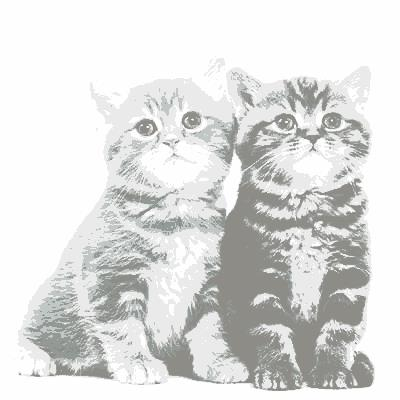
\includegraphics[width=\linewidth]{images/big/3-3-30-05}
  \caption{3x3 30 0.5}
  \label{fig:3}
\end{subfigure}

\medskip
\begin{subfigure}{0.25\textwidth}
  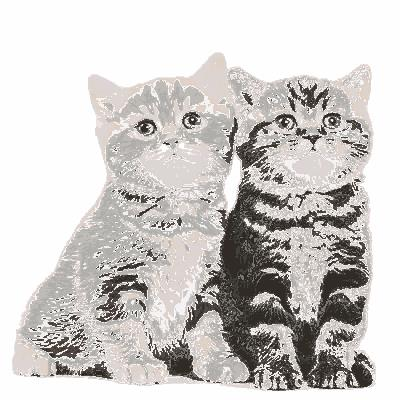
\includegraphics[width=\linewidth]{images/big/5-5-50-001}
  \caption{5x5 50 0.01}
  \label{fig:4}
\end{subfigure}\hfil % <-- added
\begin{subfigure}{0.25\textwidth}
  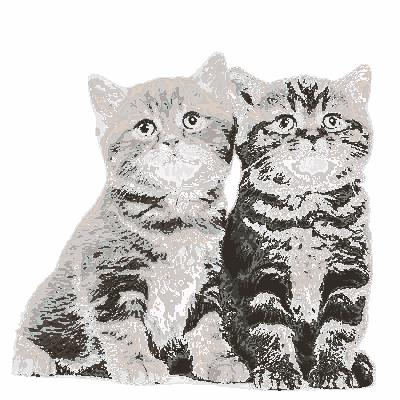
\includegraphics[width=\linewidth]{images/big/5-5-255-05}
  \caption{5x5 255 0.5}
  \label{fig:5}
\end{subfigure}
\begin{subfigure}{0.25\textwidth}
  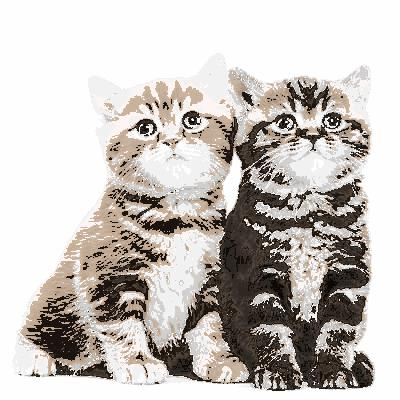
\includegraphics[width=\linewidth]{images/big/6-6-30-05}
  \caption{6x6 30 0.5}
  \label{fig:6}
\end{subfigure}\hfil % <-- added

\medskip
\begin{subfigure}{0.25\textwidth}
  
\includegraphics[width=\linewidth]{images/big/12-12-30-05}
  \caption{12x12 30 0.5}
  \label{fig:6}
\end{subfigure}
\begin{subfigure}{0.25\textwidth}
  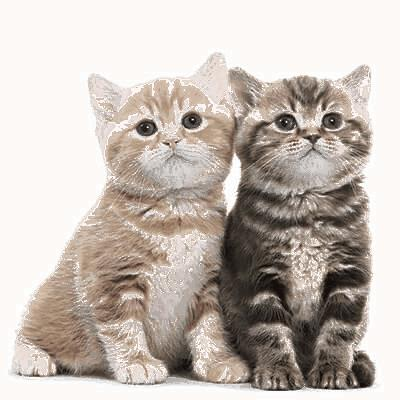
\includegraphics[width=\linewidth]{images/big/16-16-30-05}
  \caption{16x16 30 0.5}
  \label{fig:4}
\end{subfigure}\hfil % <-- added
\begin{subfigure}{0.25\textwidth}
  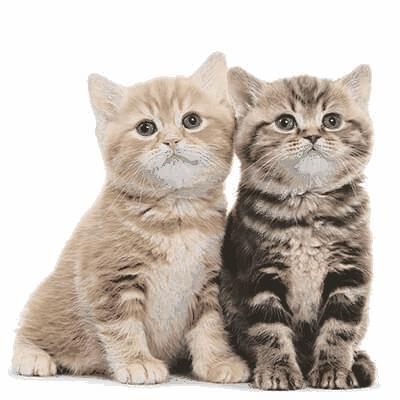
\includegraphics[width=\linewidth]{images/big/16-16-50-001}
  \caption{16x16 50 0.01}
  \label{fig:5}
\end{subfigure}\hfil % <-- added

\medskip
\begin{subfigure}{0.25\textwidth}
  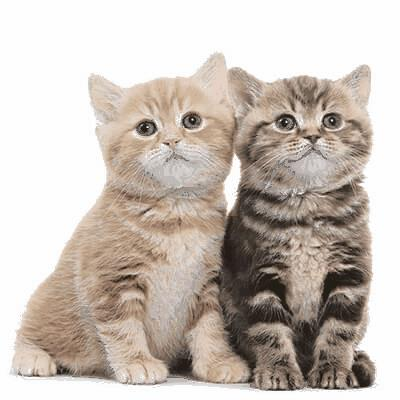
\includegraphics[width=\linewidth]{images/big/16-16-50-1}
  \caption{16x16 50 1}
  \label{fig:4}
\end{subfigure}\hfil % <-- added
\begin{subfigure}{0.25\textwidth}
  
\includegraphics[width=\linewidth]{images/big/16-16-100-05}
  \caption{16x16 100 0.5}
  \label{fig:6}
\end{subfigure}
\begin{subfigure}{0.25\textwidth}
  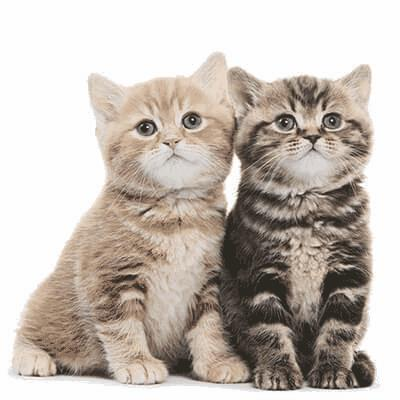
\includegraphics[width=\linewidth]{images/big/16-16-255-05}
  \caption{16x16 255 0.5}
  \label{fig:5}
\end{subfigure}\hfil % <-- added


\caption{big picture - 400x400}
\label{fig:images}
\end{figure}

\begin{figure}
    \begin{bchart}[max=500]
        \bcbar[text=original]{469}
            \smallskip
        \bcbar[text=jpg]{25.3}
            \smallskip
        \bcbar[text=b]{18.7}
            \smallskip
        \bcbar[text=c]{60.4}
            \smallskip
        \bcbar[text=d]{105}
            \smallskip
        \bcbar[text=e]{110}
            \smallskip
        \bcbar[text=f]{108}
            \smallskip
        \bcbar[text=g]{143}
            \smallskip
        \bcbar[text=h]{156}
            \smallskip
        \bcbar[text=i]{162}
            \smallskip
        \bcbar[text=j]{160}
            \smallskip
        \bcbar[text=k]{162}
            \smallskip
        \bcbar[text=l]{161}
    \end{bchart}
    \caption{Diference in size in big file in kB}
    \end{figure}
    
\begin{figure}[htb]
    \centering % <-- added
\begin{subfigure}{0.25\textwidth}
  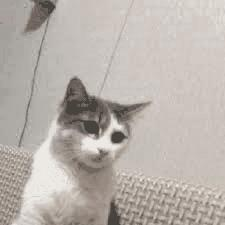
\includegraphics[width=\linewidth]{images/small/original}
  \caption{oryginal}
  \label{fig:1}
\end{subfigure}\hfil % <-- added
\begin{subfigure}{0.25\textwidth}
  
\includegraphics[width=\linewidth]{images/small/3-3-5-05}
  \caption{3x3 5 0.5}
  \label{fig:2}
\end{subfigure}\hfil % <-- added
\begin{subfigure}{0.25\textwidth}
  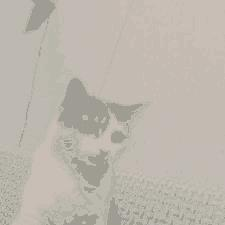
\includegraphics[width=\linewidth]{images/small/3-3-30-05}
  \caption{3x3 30 0.5}
  \label{fig:3}
\end{subfigure}

\medskip
\begin{subfigure}{0.25\textwidth}
  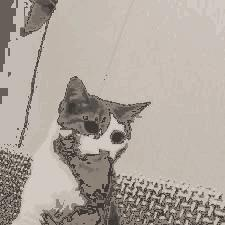
\includegraphics[width=\linewidth]{images/small/5-5-50-001}
  \caption{5x5 50 0.01}
  \label{fig:4}
\end{subfigure}\hfil % <-- added
\begin{subfigure}{0.25\textwidth}
  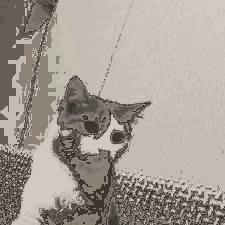
\includegraphics[width=\linewidth]{images/small/5-5-255-05}
  \caption{5x5 255 0.5}
  \label{fig:5}
\end{subfigure}
\begin{subfigure}{0.25\textwidth}
  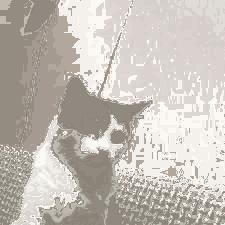
\includegraphics[width=\linewidth]{images/small/6-6-30-05}
  \caption{6x6 30 0.5}
  \label{fig:6}
\end{subfigure}\hfil % <-- added

\medskip
\begin{subfigure}{0.25\textwidth}
  
\includegraphics[width=\linewidth]{images/small/12-12-30-05}
  \caption{12x12 30 0.5}
  \label{fig:6}
\end{subfigure}
\begin{subfigure}{0.25\textwidth}
  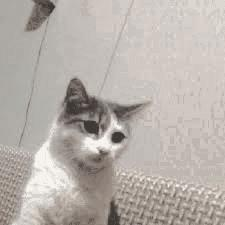
\includegraphics[width=\linewidth]{images/small/16-16-30-05}
  \caption{16x16 30 0.5}
  \label{fig:4}
\end{subfigure}\hfil % <-- added
\begin{subfigure}{0.25\textwidth}
  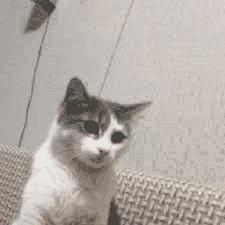
\includegraphics[width=\linewidth]{images/small/16-16-50-001}
  \caption{16x16 50 0.01}
  \label{fig:5}
\end{subfigure}\hfil % <-- added

\medskip
\begin{subfigure}{0.25\textwidth}
  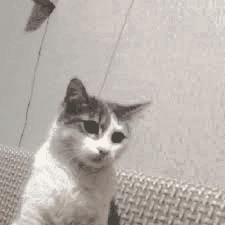
\includegraphics[width=\linewidth]{images/small/16-16-50-1}
  \caption{16x16 50 1}
  \label{fig:4}
\end{subfigure}\hfil % <-- added
\begin{subfigure}{0.25\textwidth}
  
\includegraphics[width=\linewidth]{images/small/16-16-100-05}
  \caption{16x16 100 0.5}
  \label{fig:6}
\end{subfigure}
\begin{subfigure}{0.25\textwidth}
  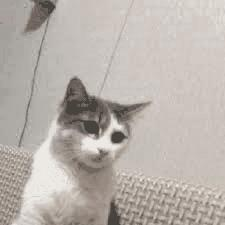
\includegraphics[width=\linewidth]{images/small/16-16-255-05}
  \caption{16x16 255 0.5}
  \label{fig:5}
\end{subfigure}\hfil % <-- added


\caption{small picture - 255x255}
\label{fig:images}
\end{figure}

\begin{figure}
    \begin{bchart}[max=150]
        \bcbar[text=original]{148}
            \smallskip
        \bcbar[text=jpg]{4.23}
            \smallskip
        \bcbar[text=b]{22.8}
            \smallskip
        \bcbar[text=c]{24.2}
            \smallskip
        \bcbar[text=d]{36}
            \smallskip
        \bcbar[text=e]{37}
            \smallskip
        \bcbar[text=f]{36.3}
            \smallskip
        \bcbar[text=g]{55.3}
            \smallskip
        \bcbar[text=h]{61.3}
            \smallskip
        \bcbar[text=i]{61.2}
            \smallskip
        \bcbar[text=j]{60.8}
            \smallskip
        \bcbar[text=k]{60.6}
            \smallskip
        \bcbar[text=l]{60.9}
    \end{bchart}    
        \caption{Diference in size in small file in kB}
    \end{figure}
    
    \begin{figure}[htb]
    \centering % <-- added
\begin{subfigure}{0.25\textwidth}
  
\includegraphics[width=\linewidth]{images/cartoon/original}
  \caption{oryginal}
  \label{fig:1}
\end{subfigure}\hfil % <-- added
\begin{subfigure}{0.25\textwidth}
  
\includegraphics[width=\linewidth]{images/cartoon/3-3-5-05}
  \caption{3x3 5 0.5}
  \label{fig:2}
\end{subfigure}\hfil % <-- added
\begin{subfigure}{0.25\textwidth}
  
\includegraphics[width=\linewidth]{images/cartoon/3-3-30-05}
  \caption{3x3 30 0.5}
  \label{fig:3}
\end{subfigure}

\medskip
\begin{subfigure}{0.25\textwidth}
  
\includegraphics[width=\linewidth]{images/cartoon/5-5-50-001}
  \caption{5x5 50 0.01}
  \label{fig:4}
\end{subfigure}\hfil % <-- added
\begin{subfigure}{0.25\textwidth}
  
\includegraphics[width=\linewidth]{images/cartoon/5-5-255-05}
  \caption{5x5 255 0.5}
  \label{fig:5}
\end{subfigure}
\begin{subfigure}{0.25\textwidth}
  
\includegraphics[width=\linewidth]{images/cartoon/6-6-30-05}
  \caption{6x6 30 0.5}
  \label{fig:6}
\end{subfigure}\hfil % <-- added

\medskip
\begin{subfigure}{0.25\textwidth}
  
\includegraphics[width=\linewidth]{images/cartoon/12-12-30-05}
  \caption{12x12 30 0.5}
  \label{fig:6}
\end{subfigure}
\begin{subfigure}{0.25\textwidth}
  
\includegraphics[width=\linewidth]{images/cartoon/16-16-30-05}
  \caption{16x16 30 0.5}
  \label{fig:4}
\end{subfigure}\hfil % <-- added
\begin{subfigure}{0.25\textwidth}
  
\includegraphics[width=\linewidth]{images/cartoon/16-16-50-001}
  \caption{16x16 50 0.01}
  \label{fig:5}
\end{subfigure}\hfil % <-- added

\medskip
\begin{subfigure}{0.25\textwidth}
  
\includegraphics[width=\linewidth]{images/cartoon/16-16-50-1}
  \caption{16x16 50 1}
  \label{fig:4}
\end{subfigure}\hfil % <-- added
\begin{subfigure}{0.25\textwidth}
  
\includegraphics[width=\linewidth]{images/cartoon/16-16-100-05}
  \caption{16x16 100 0.5}
  \label{fig:6}
\end{subfigure}
\begin{subfigure}{0.25\textwidth}
  
\includegraphics[width=\linewidth]{images/cartoon/16-16-255-05}
  \caption{16x16 255 0.5}
  \label{fig:5}
\end{subfigure}\hfil % <-- added


\caption{cartoon picture}
\label{fig:images}
\end{figure}

\begin{figure}
    \begin{bchart}[max=200]
        \bcbar[text=original]{192}
            \smallskip
        \bcbar[text=jpg]{13.1}
            \smallskip
        \bcbar[text=b]{23.9}
            \smallskip
        \bcbar[text=c]{13.9}
            \smallskip
        \bcbar[text=d]{32.5}
            \smallskip
        \bcbar[text=e]{31.7}
            \smallskip
        \bcbar[text=f]{36.1}
            \smallskip
        \bcbar[text=g]{49}
            \smallskip
        \bcbar[text=h]{56.5}
            \smallskip
        \bcbar[text=i]{57.9}
            \smallskip
        \bcbar[text=j]{58.4}
            \smallskip
        \bcbar[text=k]{58.2}
            \smallskip
        \bcbar[text=l]{57.8}
    \end{bchart} 
            \caption{Diference in size in cartoon file in kB}
    \end{figure}

Ćwiczenie z siecią CAN było całkiem proste i przyjemne. Bardzo łatwo można skonfigurować pliki z zadeklarowanymi zmiennymi, żeby przesyłać dane między sterownikami. Nie wiemy za to, czy konfigurowanie sterownika do pracy w sieci CAN jest równie proste, ponieważ pracowaliśmy na przygotowanych wcześniej projektach.
\end{document}
% Koniec wieńczy dzieło.
